The electron reconstruction, identification, and isolation play a crucial role for many ATLAS analysis.
The electrons\footnote{The electrons and positron are referred to as electrons.} leave tracks in the inner detector and energy deposits in the ECAL.
The reconstruction algorithm combines the signals in the calorimeter and the tracks in the inner detector to defined the electron candidates.
The reconstructed candidates are identified as electrons based on a likelihood discrimination which distinguishes the electron candidates from the hadrons, non-prompt electrons originating from photon conversions, and heavy flavor hadron decays.
Additionally, the electron candidates are required to be isolated to further distinguish the signal and the background objects.
The electron efficiency measurements are performed based on the tag-and-probe method using the $Z \to eel$ and $J/\psi \to ee$ samples.
This chapter describes the basic concept of the electron reconstruction and identification briefly and will focus on the electron isolation measurement using the $Z \to ee$ samples only.

%%%
%%%
%%%

\section{Tag-and-probe method}
\label{sec:app_tag_and_probe_method}
In order to measure the electron efficiency, the tag-and-probe method and an unbiased and clean electron enriched $Z \to ee$ or $J/\psi \to ee$ sample are used.
A strict selection criteria are applied on one of the electron candidates (called ``tag'') together with the requirements based on the invariant mass window allows for a loose pre-identification of the other electron candidate (``probe'').
Only the probe electrons are used in the electron efficiency measurement after subtracting the background.
Each the valid combination of electron tag-and-probe pairs in the events is considered, therefore, an electron can be the tag in one tag-and-probe pair and the probe in another.
There are two background estimation methods using $Z \to ee$ events: the $Z_{mass}$ and the $Z_{iso}$ methods.
The $Z_{mass}$ method constructs background templates by reverting the identification and isolation requirements.
The background templates are then normalized using the events in the side band region.
The $Z_{iso}$ method constructs a background template by reverting the identification requirements only.
The background templates are then normalized to the background dominated upper end of the $E_\mathrm{T}^\mathrm{cone0.3}$ isolation distribution.
Figure~\ref{fig:app_electron_isolation_Zee_background_subtraction_methods} shows the background estimations using the $Z_{mass}$ and $Z_{iso}$ methods.

\begin{figure}[htbp]
    \begin{subfigure}[b]{0.48\textwidth}
        \begin{center}
            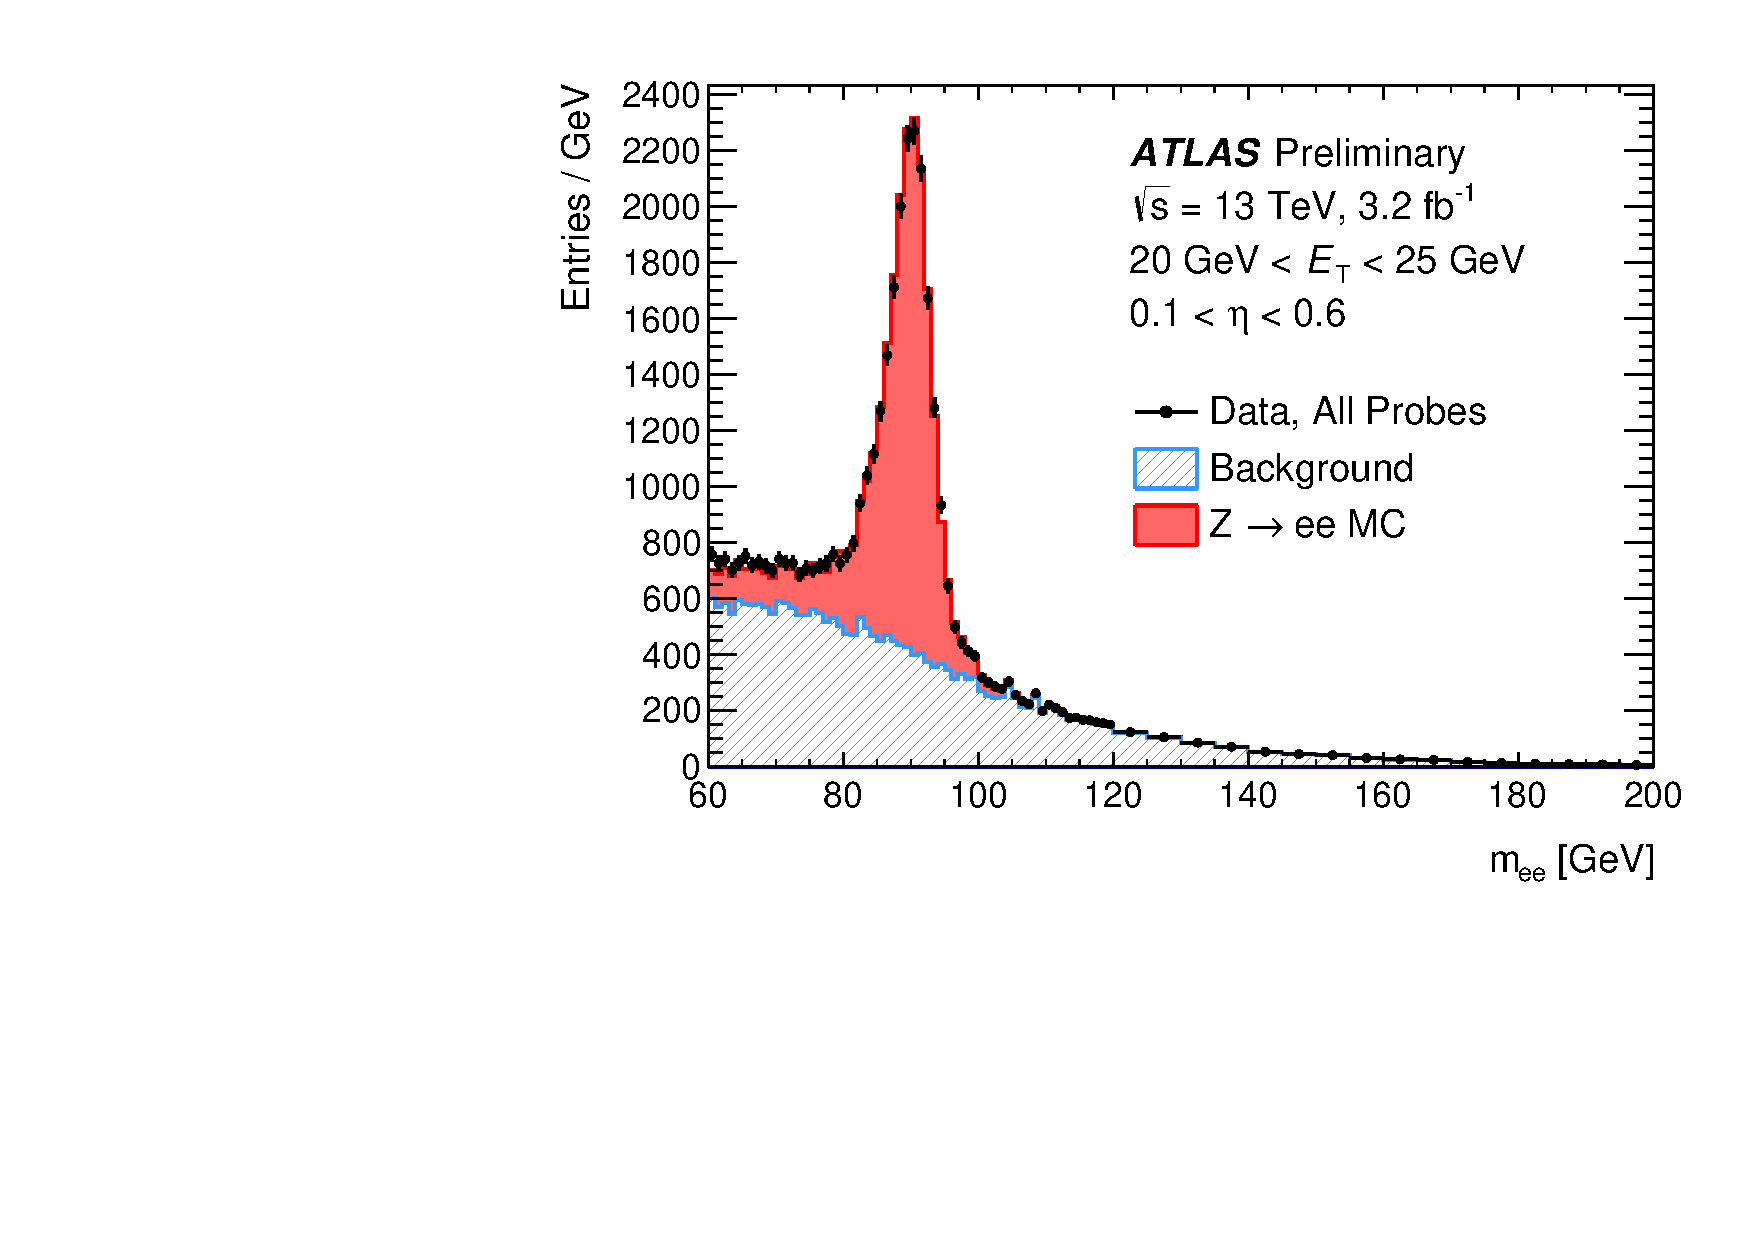
\includegraphics[scale=0.35]{fig_03a.pdf}
            \caption{The $Z_{mass}$ method}
        \end{center}
    \end{subfigure}
    \begin{subfigure}[b]{0.48\textwidth}
        \begin{center}
            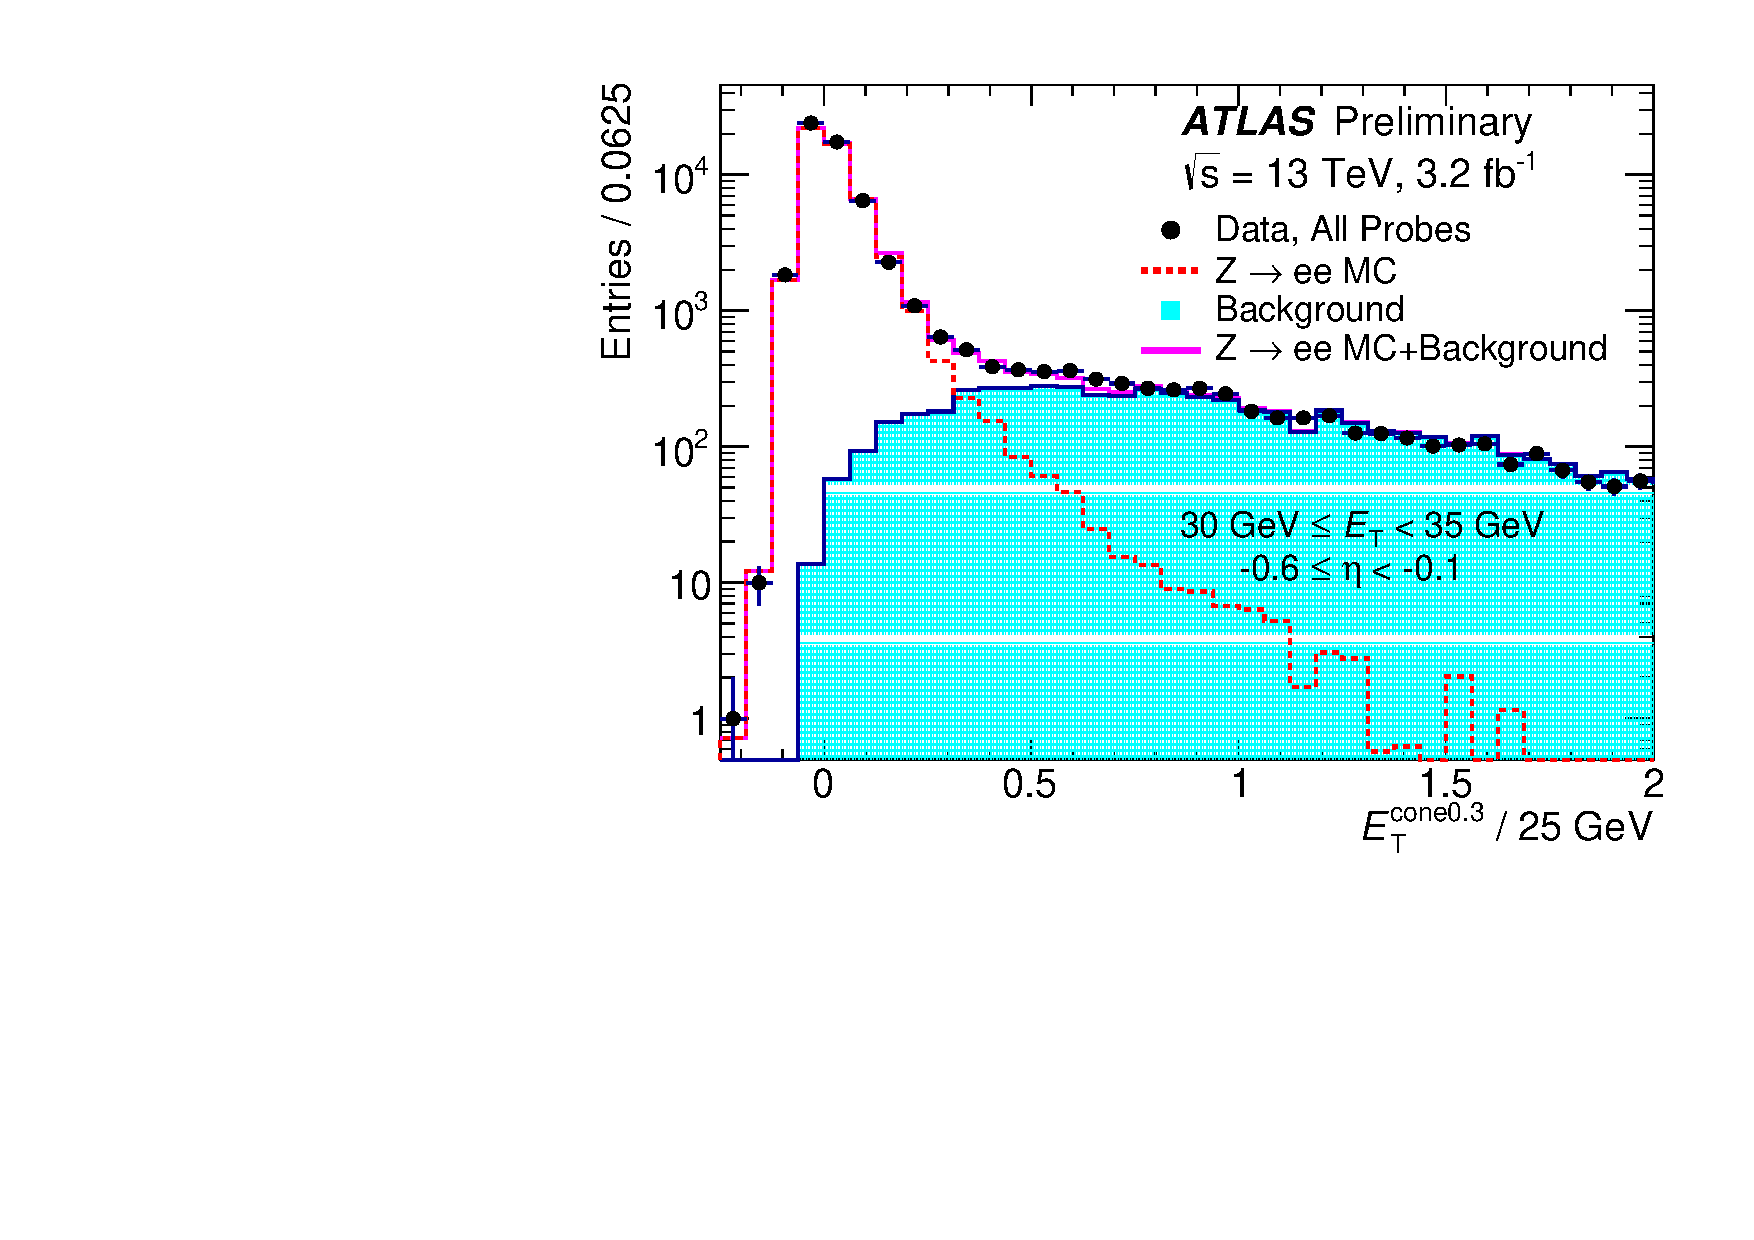
\includegraphics[scale=0.35]{fig_04a.pdf}
            \caption{The $Z_{iso}$ method}
        \end{center}
    \end{subfigure}
    \caption{Illustration of the background estimations use (a) the $Z_{mass}$ and (b) the $Z_{iso}$ methods~\cite{ATLAS:2016iqc}.}
    \label{fig:app_electron_isolation_Zee_background_subtraction_methods}
\end{figure}

The electrons in $J/\Psi$ samples have prompt and non-prompt components.
The prompt electron comes from the prompt production of $J/\Psi$ which comes from the $pp$ collisions and the non-prompt one arises from the non-prompt production of $J/\Psi$ which comes from $b$ decay.
The prompt electron is expected more isolated than the non-prompt one.
By using this distinguish feature, a tag-and-probe pair can be constructed.
There are two background estimation methods: short-$\tau$ and $\tau$-fit methods.
The short-$\tau$ method uses the events with short pseudo-proper time to find the prompt electron and the $\tau$-fit method considers the full $\tau$-range to extract the non-prompt electron by fitting the pseudo-proper time distribution.
Figure~\ref{fig:app_electron_isolation_JPsi_background_subtraction_methods} shows the background estimations using the short-$\tau$ and $\tau$-fit methods.

\begin{figure}[htbp]
    \begin{subfigure}[b]{0.48\textwidth}
        \begin{center}
            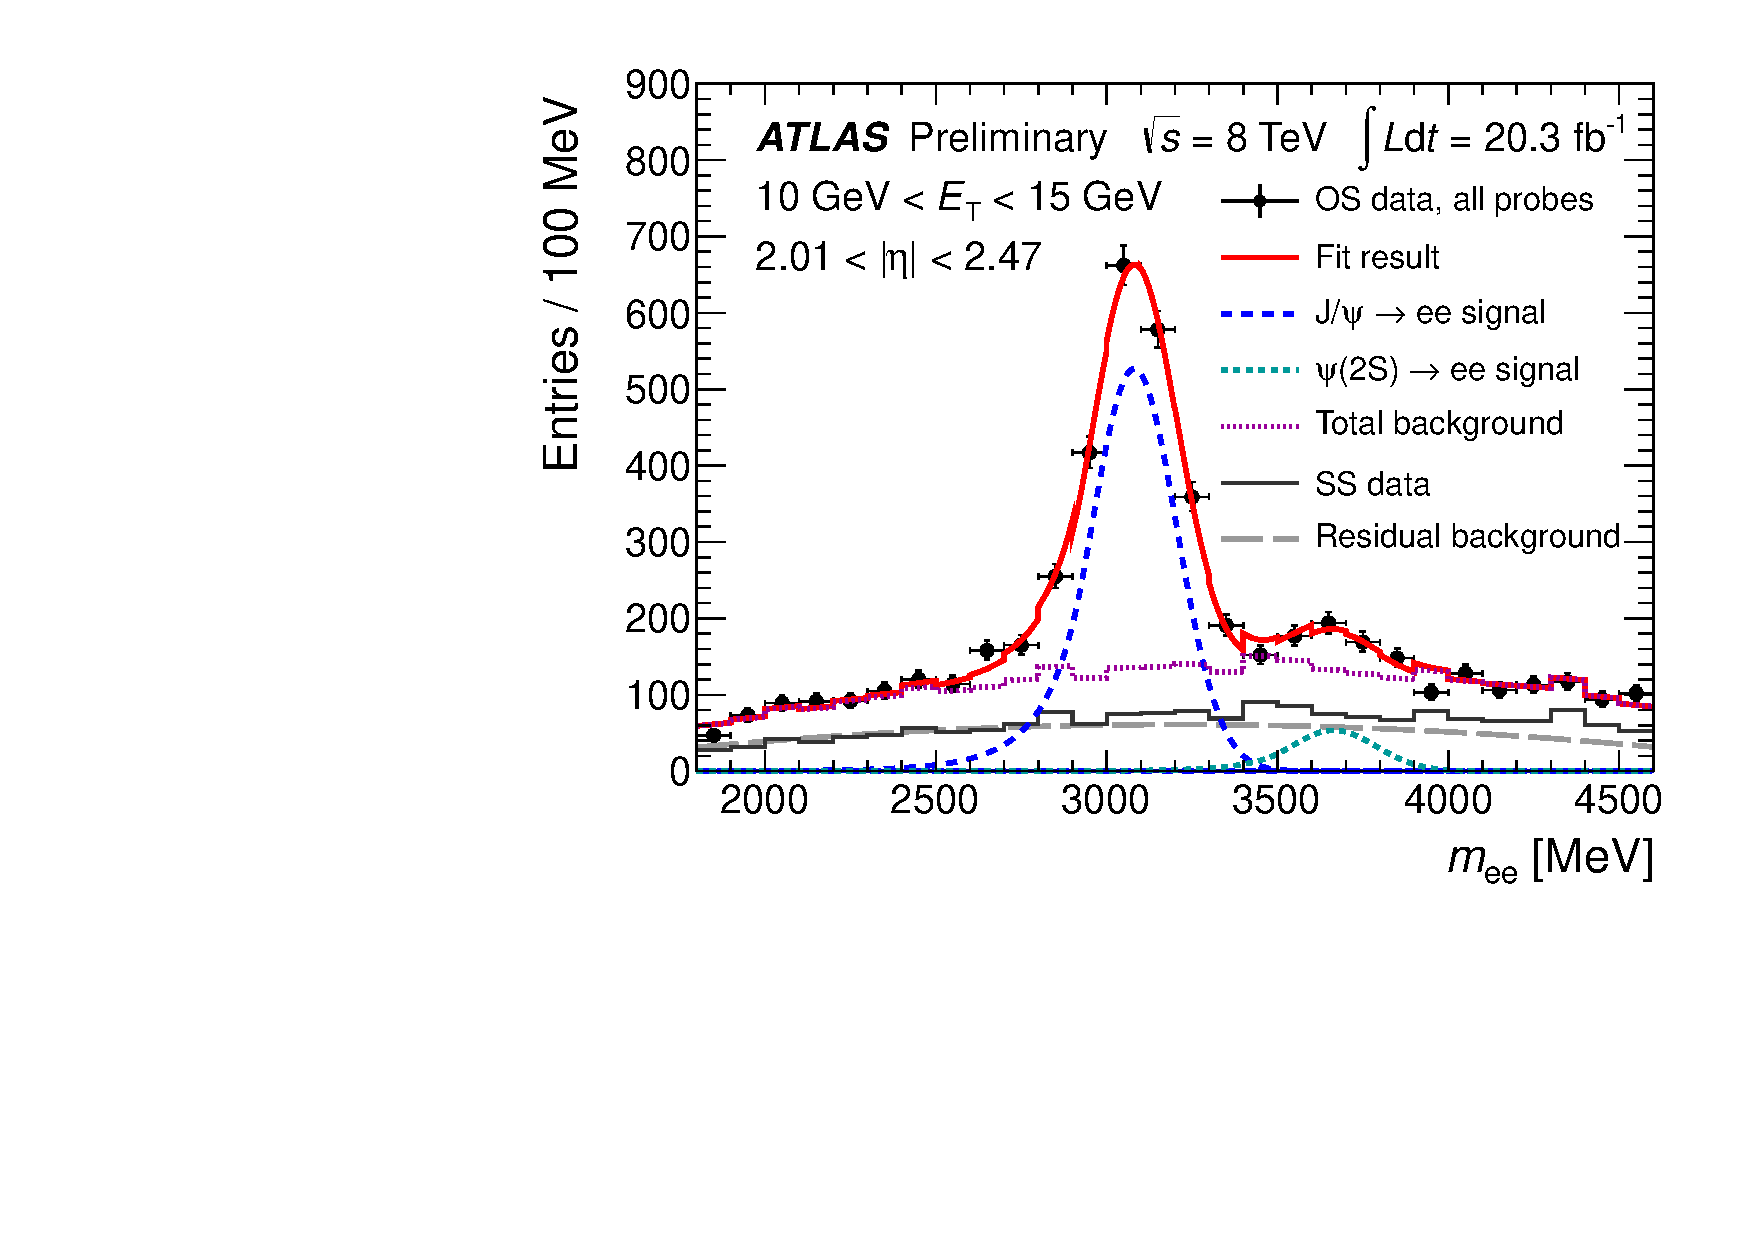
\includegraphics[scale=0.35]{fig_07a.pdf}
            \caption{The short-$\tau$ method}
        \end{center}
    \end{subfigure}
    \begin{subfigure}[b]{0.48\textwidth}
        \begin{center}
            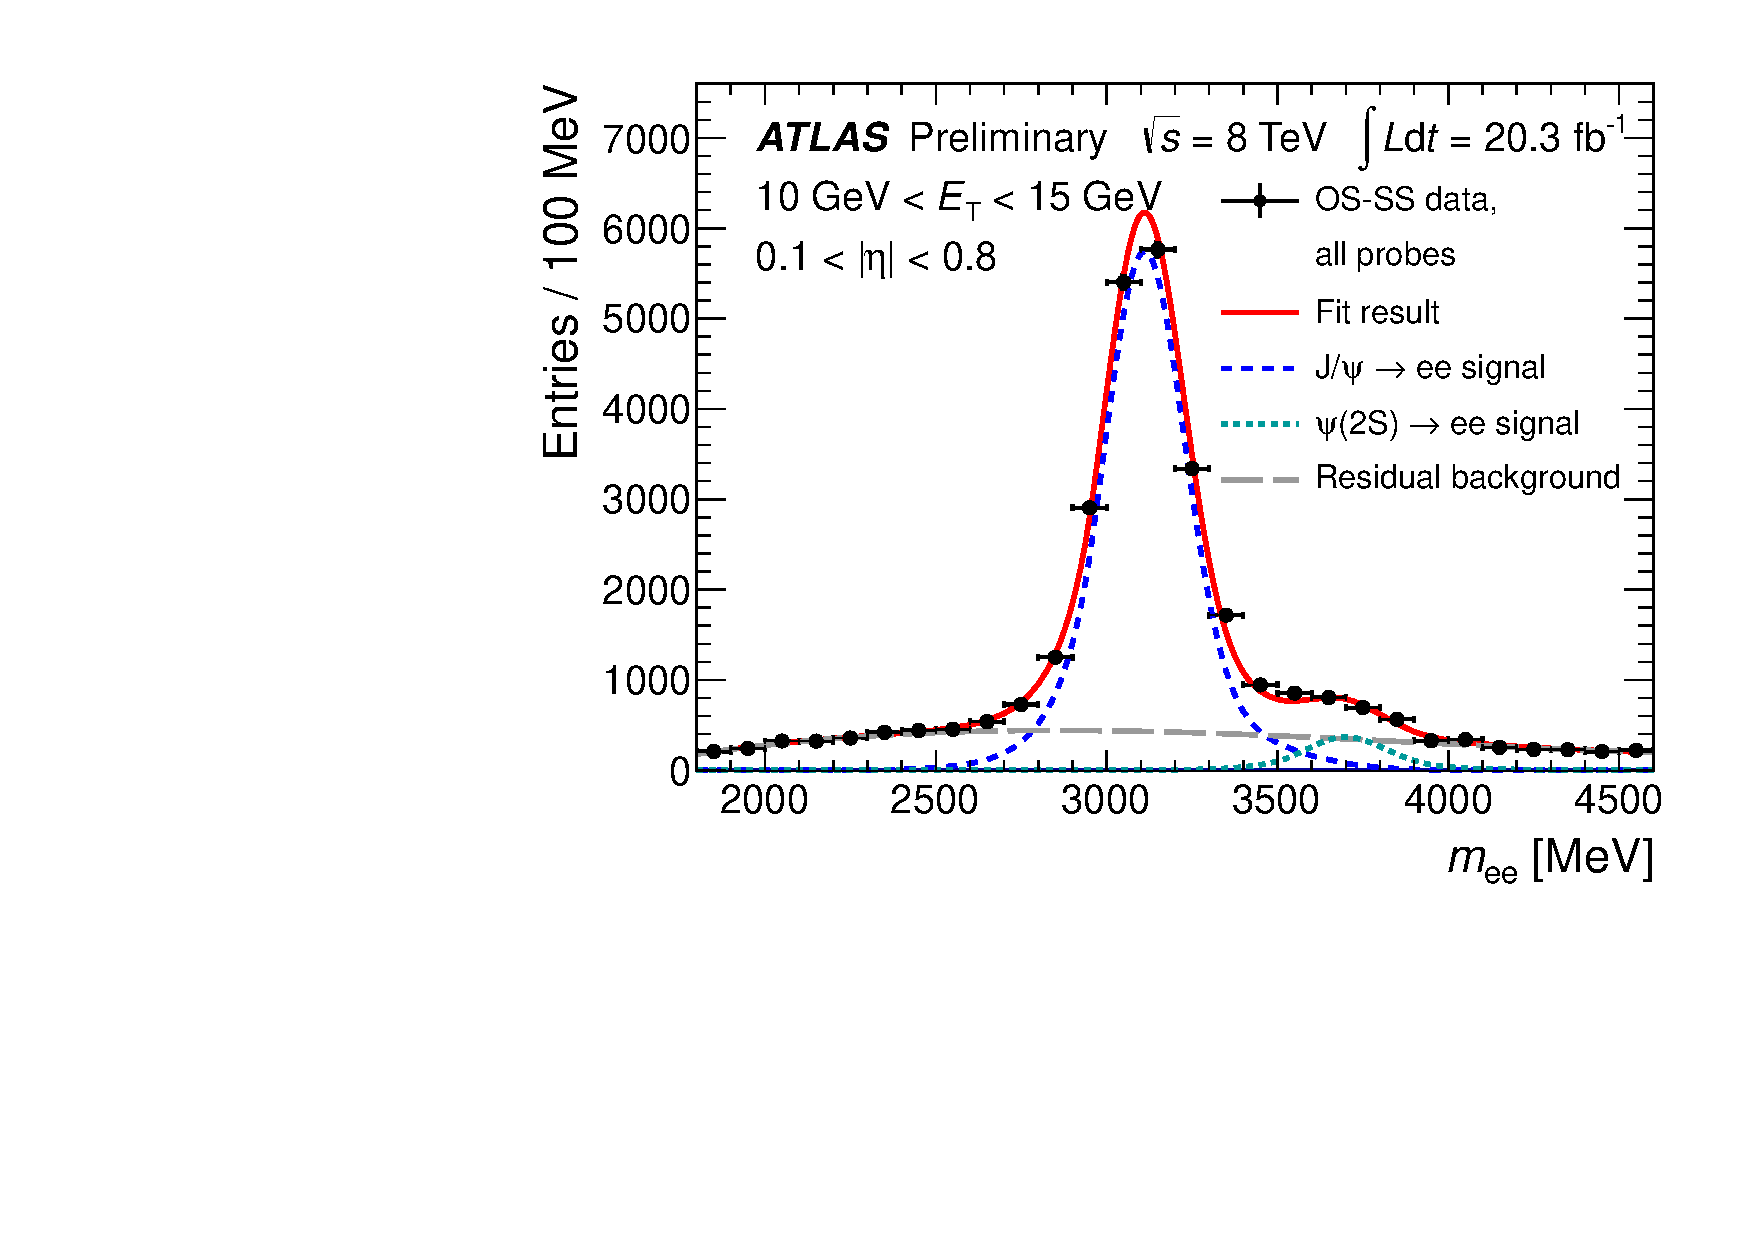
\includegraphics[scale=0.35]{fig_08a.pdf}
            \caption{The $\tau$-fit method}
        \end{center}
    \end{subfigure}
    \caption{Illustration of the background estimations use (a) the short-$\tau$ and (b) the $\tau$-fit methods~\cite{Aaboud:2016vfy}.}
    \label{fig:app_electron_isolation_JPsi_background_subtraction_methods}
\end{figure}

In the electron isolation, the $Z \to ee$ sample and the $Z_{mass}$ method are used.

%%%
%%%
%%%

\section{Electron reconstruction and identification}
\label{sec:app_electron_reconstruction_and_identification}
The electrons candidates are reconstructed in the central region of the ATLAS detector ($|\eta| < 2.47$) using information from the inner detector and ECAL.
Then the electron identification (ID) algorithms are used to distinguish the signal or background-like candidates based on multivariate likelihood discriminant.
The signal-like electrons should be prompt and isolated.
The background-like electrons coming from photon conversions, hadronic jets misidentification, and heavy flavor decays are non-prompt.
The IBL added for Run-2 can provide good discrimination between electrons and converted photons.
Three electron ID operating points \texttt{Tight}, \texttt{Medium}, and \texttt{Loose} are provided.
The \texttt{Tight} ID provides the highest background rejection power, the \texttt{Loose} has the lowest background rejection power, and \texttt{Medium} ID in between.
Figure~\ref{fig:app_electron_isolation_schematic_view_of_electron_reco_ID} shows the schematic view of the electron reconstruction and identification.
The electron reconstruction and identification efficiencies for 2016 data corresponding 33.9~\ifb are shown in Fig.~\ref{fig:app_electron_isolation_2016_electron_ID_efficiencies}.

\begin{figure}[htbp]
    \begin{center}
        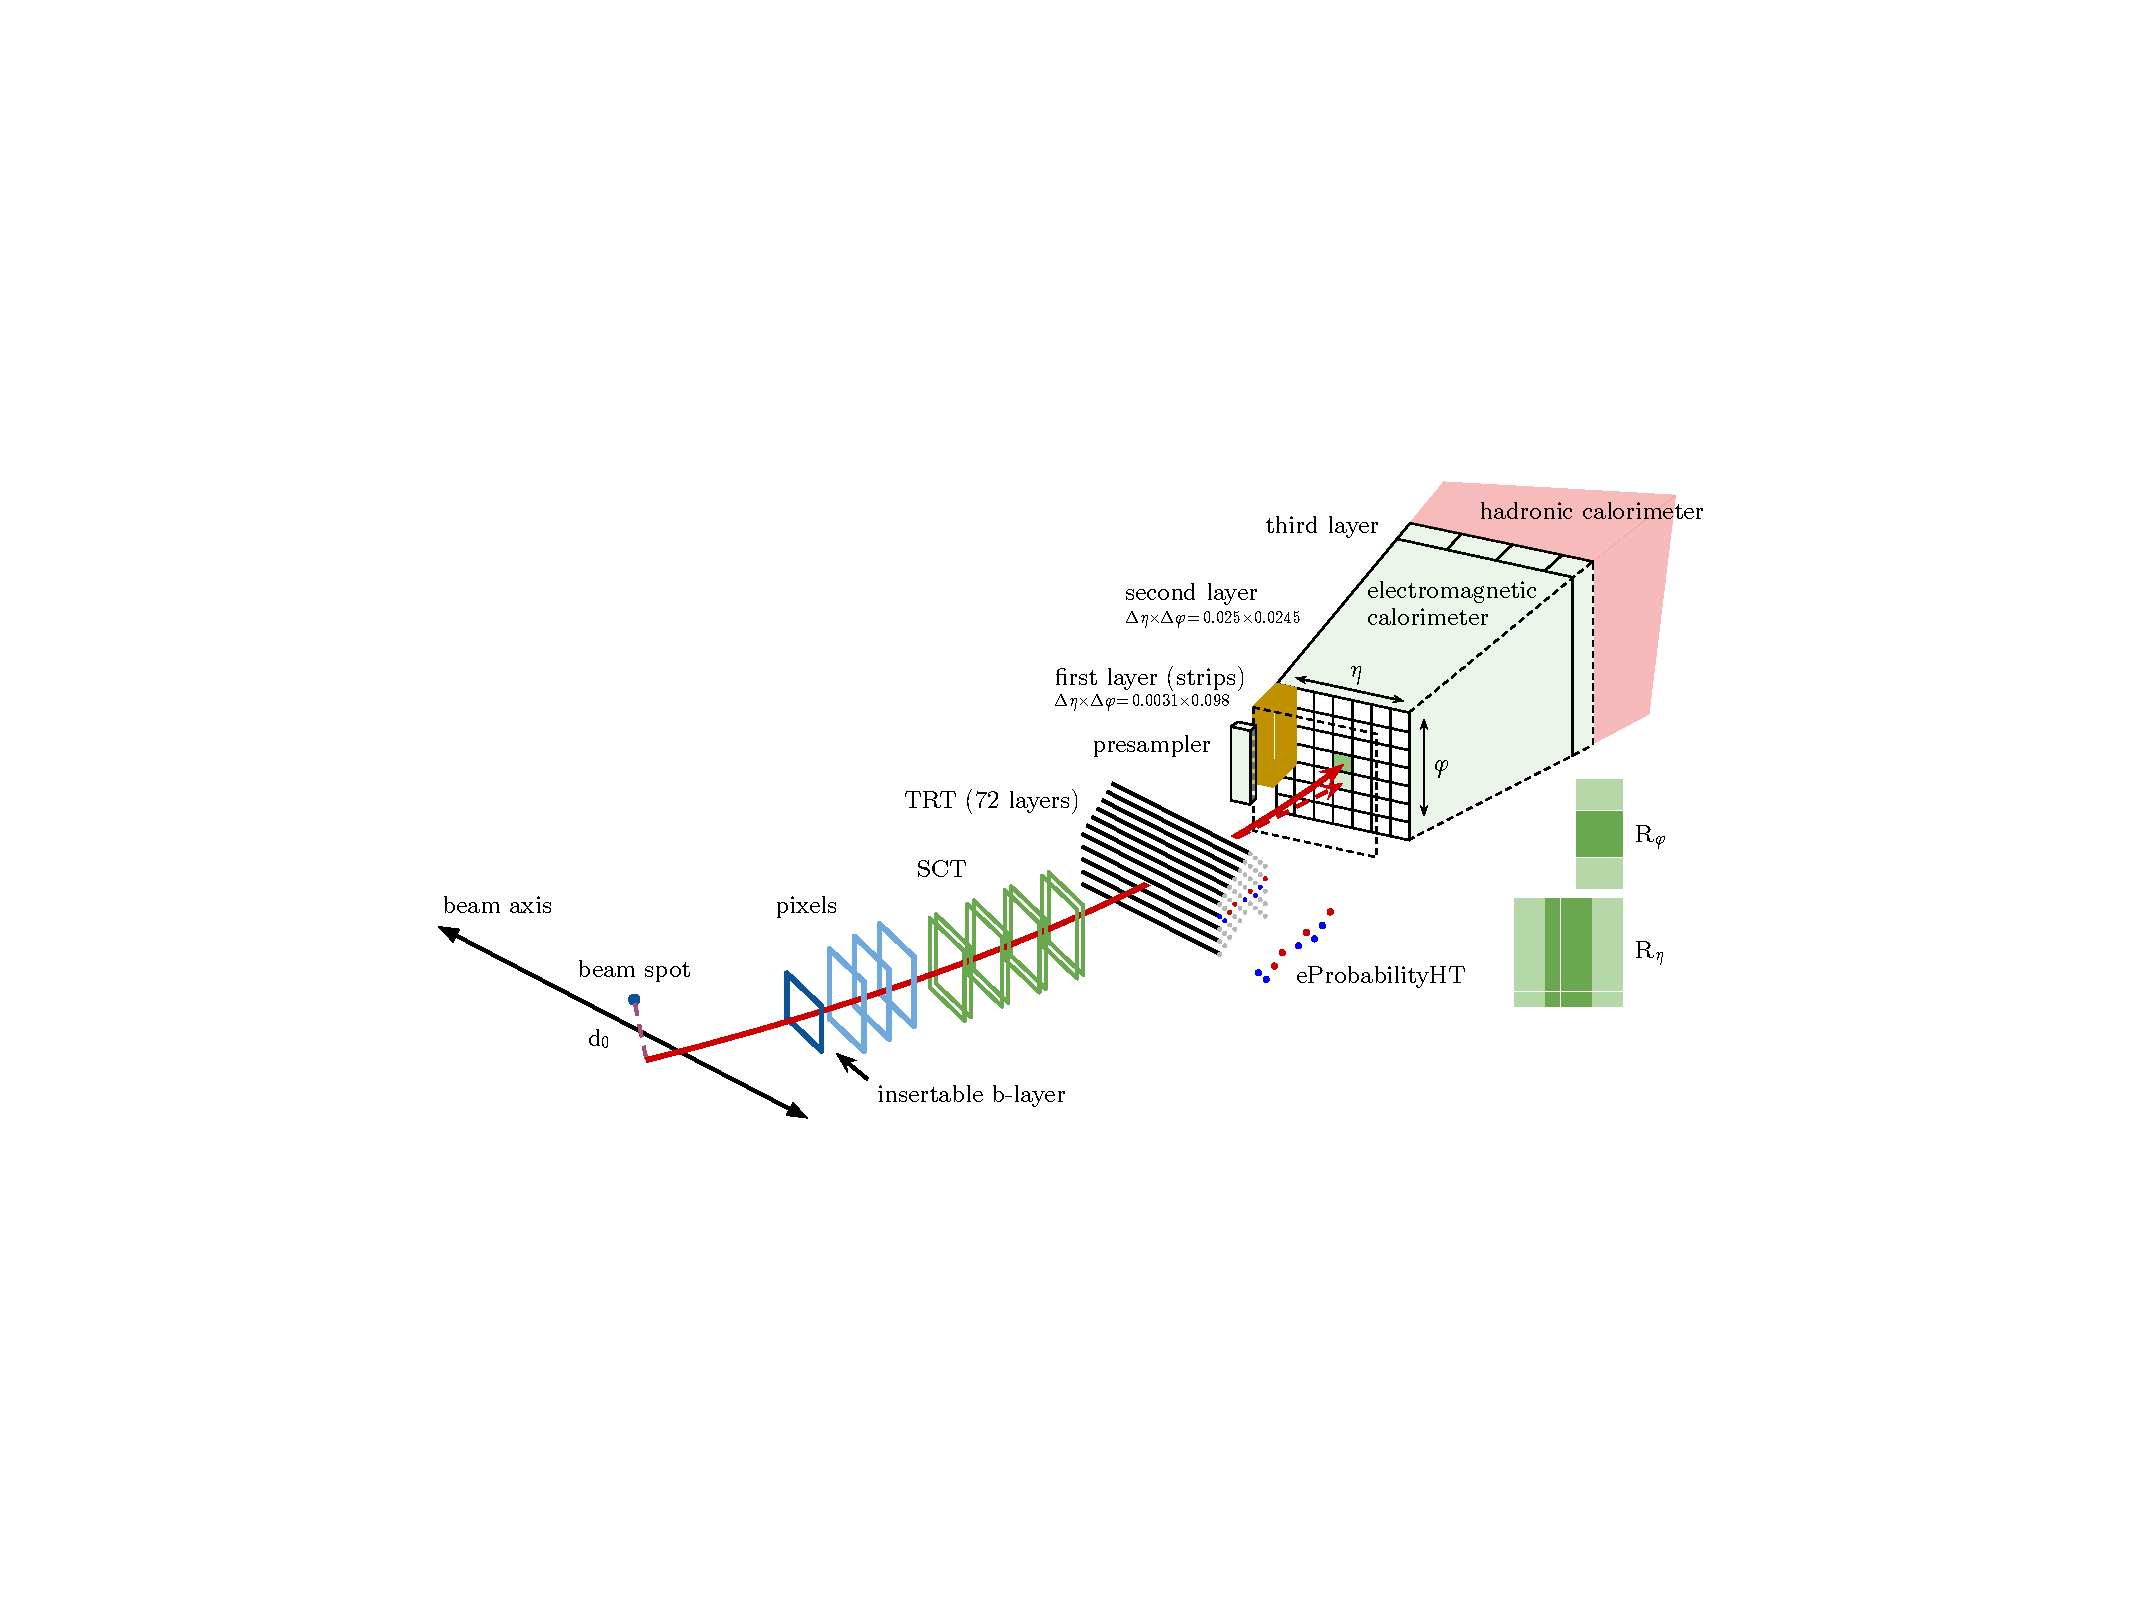
\includegraphics[scale=0.6]{figaux_03.pdf}
        \caption{The schematic view of the electron reconstruction and identification~\cite{ATLAS:2016iqc}.}
        \label{fig:app_electron_isolation_schematic_view_of_electron_reco_ID}
    \end{center}
\end{figure}

\begin{figure}[htbp]
    \begin{subfigure}[b]{0.32\textwidth}
        \begin{center}
            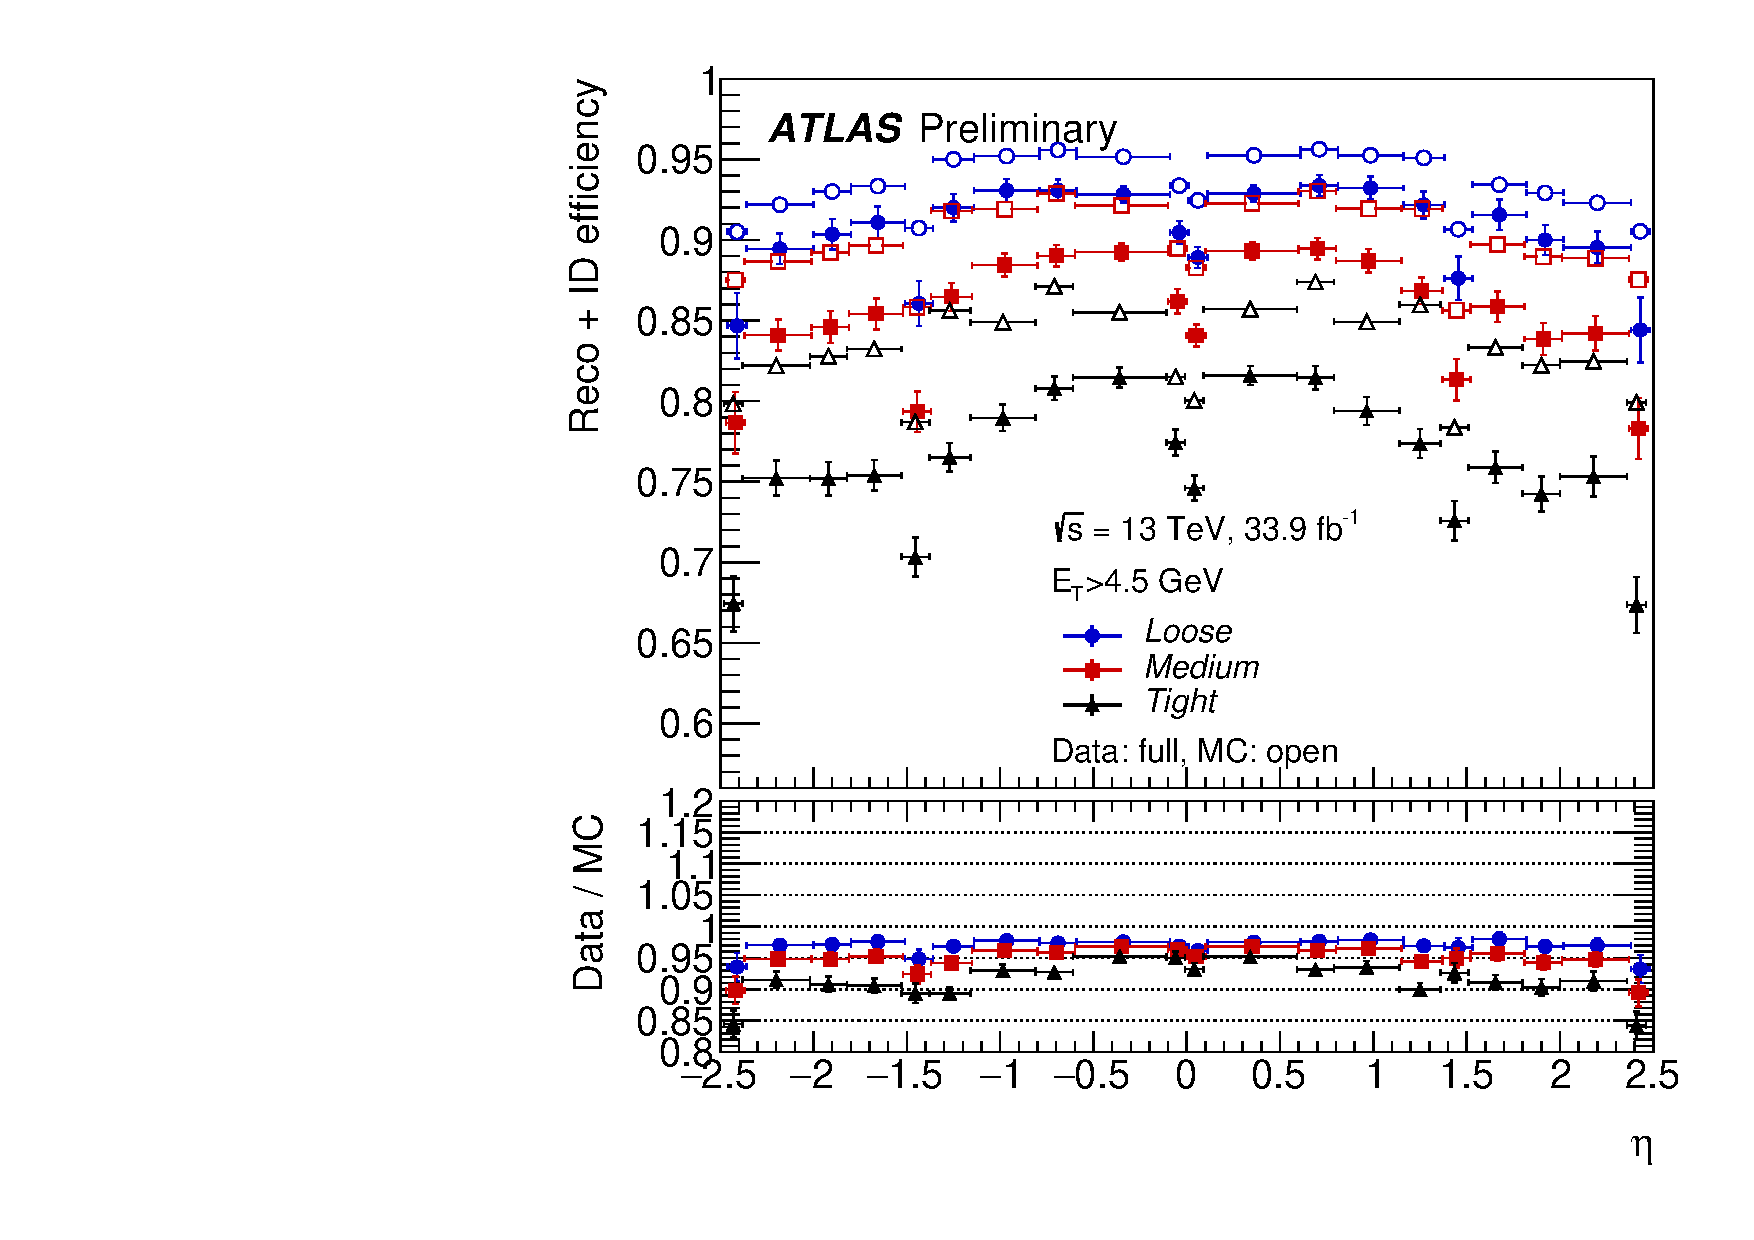
\includegraphics[scale=0.23]{fig_01.pdf}
            \caption{}
        \end{center}
    \end{subfigure}
    \begin{subfigure}[b]{0.32\textwidth}
        \begin{center}
            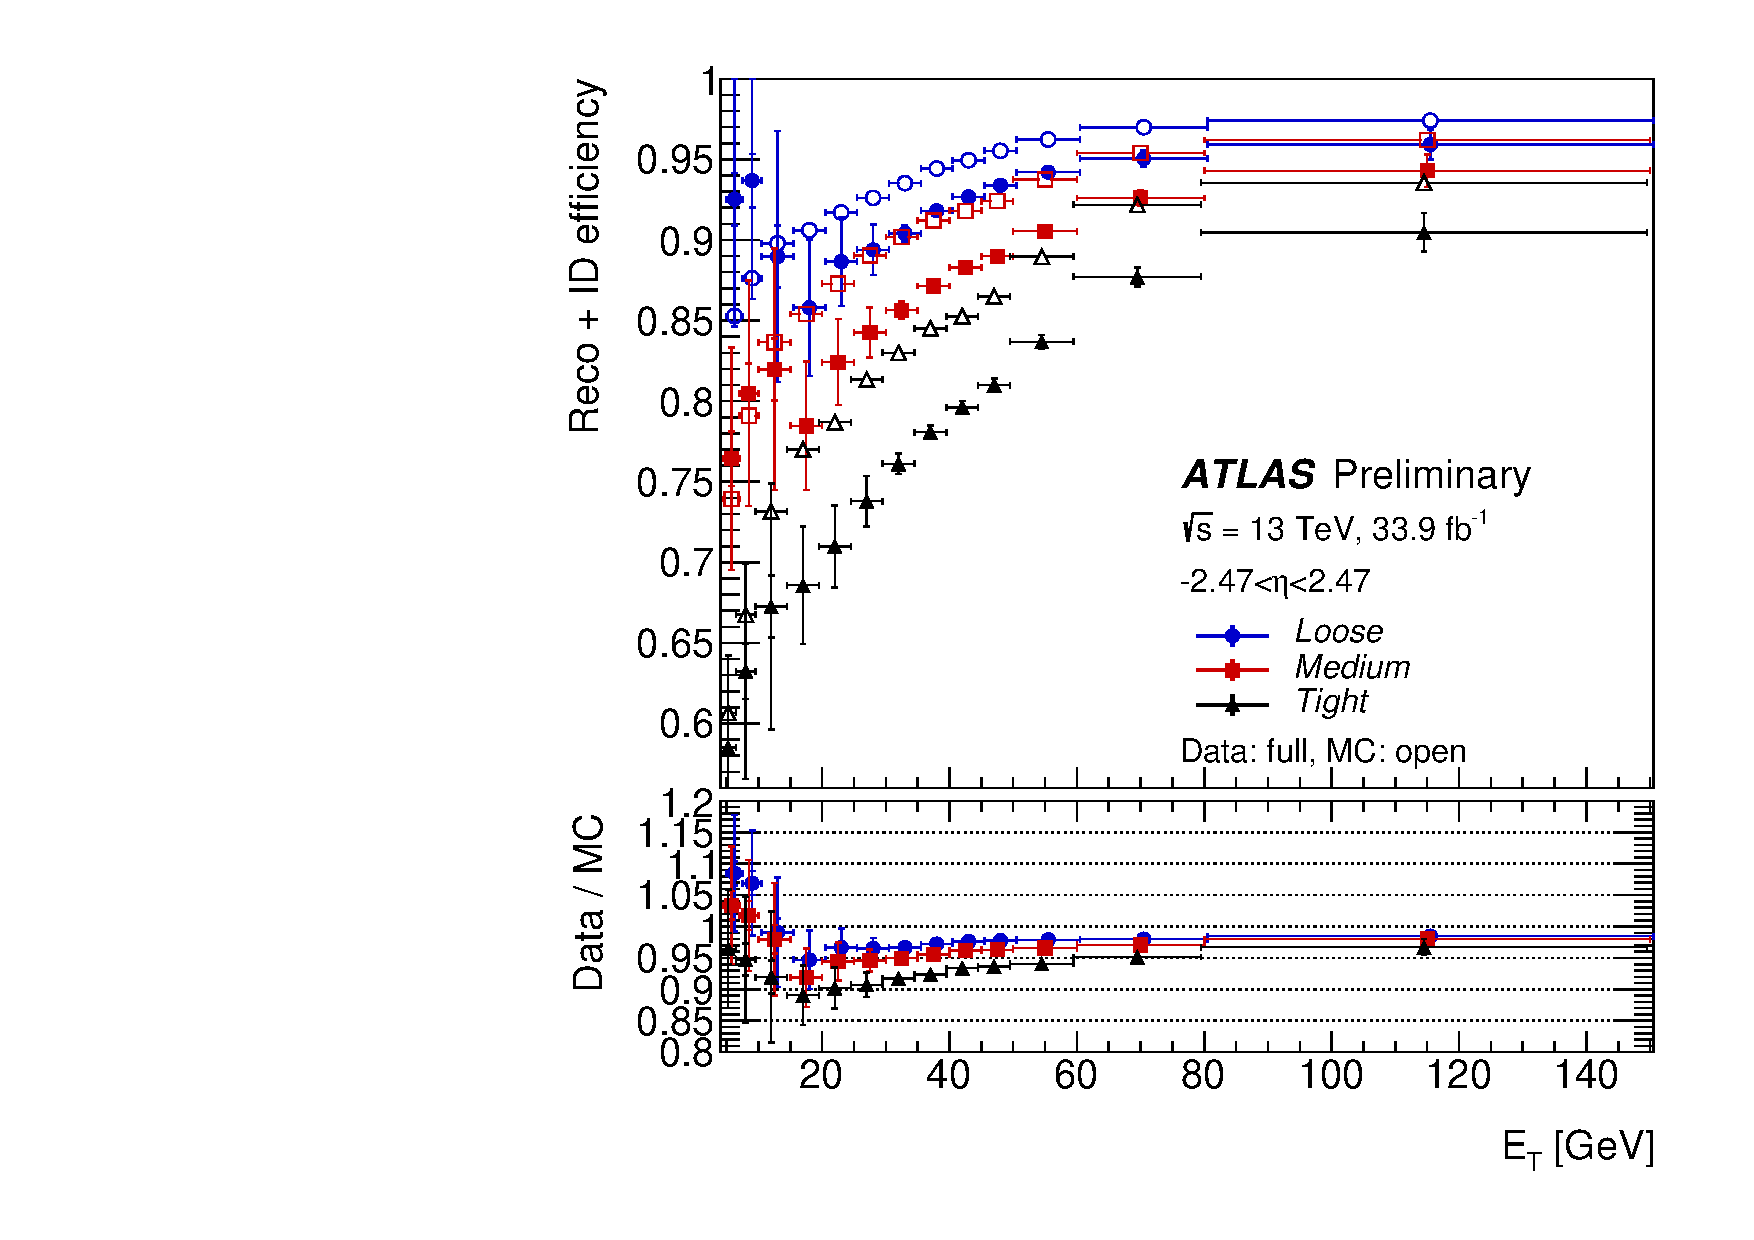
\includegraphics[scale=0.23]{fig_02.pdf}
            \caption{}
        \end{center}
    \end{subfigure}
    \begin{subfigure}[b]{0.32\textwidth}
        \begin{center}
            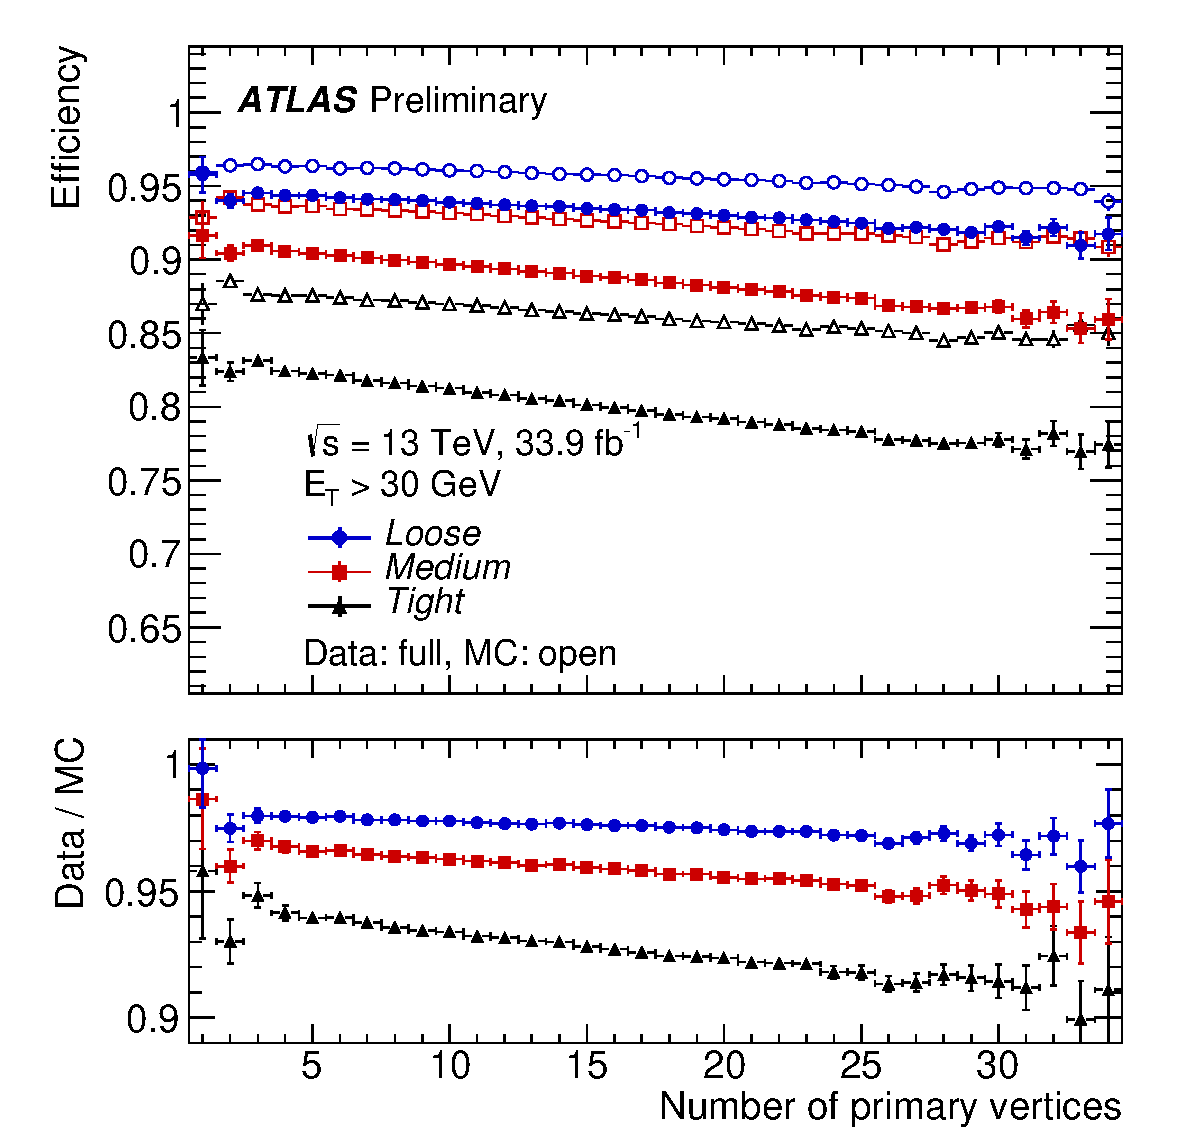
\includegraphics[scale=0.23]{fig_03.pdf}
            \caption{}
        \end{center}
    \end{subfigure}
    \caption{The electron reconstruction and identification efficiencies as a function of (a) $\eta$ and (b) \met~\cite{ATLAS:EGAM-2017-003}.
    The electron identification efficiency as a function of (c) the number of reconstructed primary vertices~\cite{ATLAS:EGAM-2016-005}.}
    \label{fig:app_electron_isolation_2016_electron_ID_efficiencies}
\end{figure}

%%%
%%%
%%%

\section{Electron isolation}
\label{sec:app_electron_isolation}
The electrons produced in the LHC $pp$ collisions cover a wide range of \met from a few {\GeV} to several {\TeV}.
The reconstructed electrons suffer large backgrounds from misidentified hadrons, photon conversions, and heavy-flavor decays.
In order to further discriminate signal and background, most analyses require electrons to be isolated in addition to the identification criteria.
The background electrons are produced in association with other objects such as jets, therefore they have larger values of isolation. 
However, the signal electrons tend to have low values of isolation as they are uncorrelated with other jet activities in the event.
The isolation variables quantify the energy deposited in a cone centered around the electron candidates and allow to disentangle prompt electrons from non-isolated electrons.
Hence, the electron isolation is a very powerful tool to reject backgrounds.
Two discriminating variables have been designed for that purpose: a calorimetric isolation energy $E_\mathrm{T}^\mathrm{cone\ 0.2}$ and a track isolation $p_\mathrm{T}^\mathrm{varcone\ 0.2}$.
The $E_\mathrm{T}^\mathrm{cone\ 0.2}$ is defined as the sum of transverse energies of topological clusters~\cite{Aad:2016upy} within a cone of $\Delta R = 0.2$ around the candidate electron cluster and excluding the contribution in a region $\Delta \eta \times \Delta \phi = 0.125 \times 0.175$ centered around the electron cluster barycentre.
Only clusters with positive $E_\mathrm{T}$ are considered in the sum.
The energy leakage outside the clusters, the pileup contributions, and the underlying event activity are corrected. 
The $p_\mathrm{T}^\mathrm{varcone\ 0.2}$ is defined as the sum of transverse momenta of all tracks within a cone of $\Delta R = \mathrm{min}(0.2, 10~{\GeV}/E_\mathrm{T})$ around the candidate electron track and originating from the reconstructed primary vertex of the hard collision.
The track must satisfies $E_\mathrm{T} > 1$~{\GeV}, $|\Delta z_{0} \sin \theta| < 3$~mm, and $n_\mathrm{Si} \ge 7$, $n_\mathrm{Si}^\mathrm{hole} \le 2$, $n_\mathrm{pixel}^\mathrm{hole} \le 1$, and $n_\mathrm{mod}^\mathrm{sh} \le 1$, where $n_\mathrm{Si}^\mathrm{hole}$ and $n_\mathrm{pixel}^\mathrm{hole}$ are the number of missing hits in the silicon and pixel detector respectively and $n_\mathrm{mod}^\mathrm{sh}$ is the number of hits in the silicon detector assigned to more than one track.
The distributions of $E_\mathrm{T}^\mathrm{cone\ 0.2}$ and $p_\mathrm{T}^\mathrm{varcone\ 0.2}$ are shown in Fig.~\ref{fig:app_electron_isolation_ETcone20_PTvarcone20}.

\begin{figure}[htbp]
    \begin{subfigure}[b]{0.48\textwidth}
        \begin{center}
            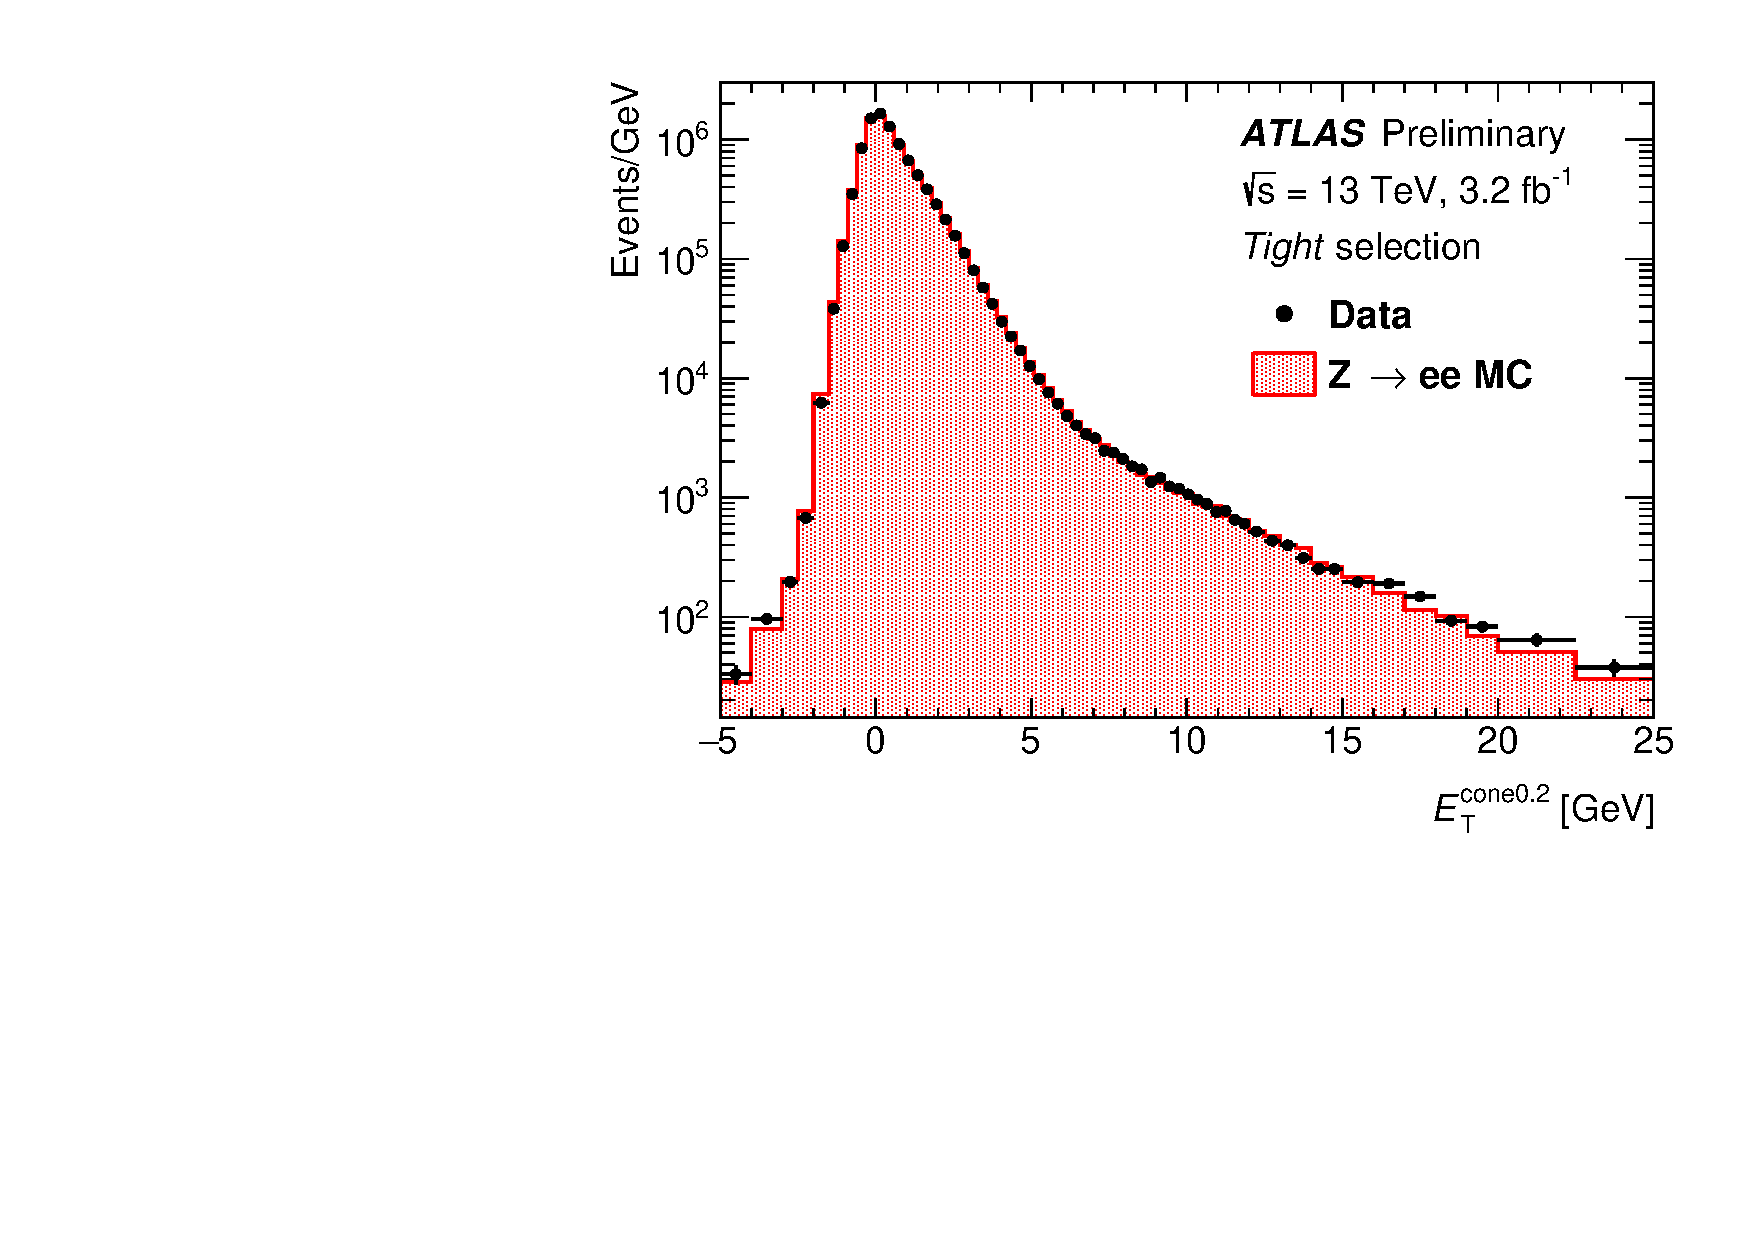
\includegraphics[scale=0.35]{fig_02a.pdf}
            \caption{$E_\mathrm{T}^\mathrm{cone\ 0.2}$}
        \end{center}
    \end{subfigure}
    \begin{subfigure}[b]{0.48\textwidth}
        \begin{center}
            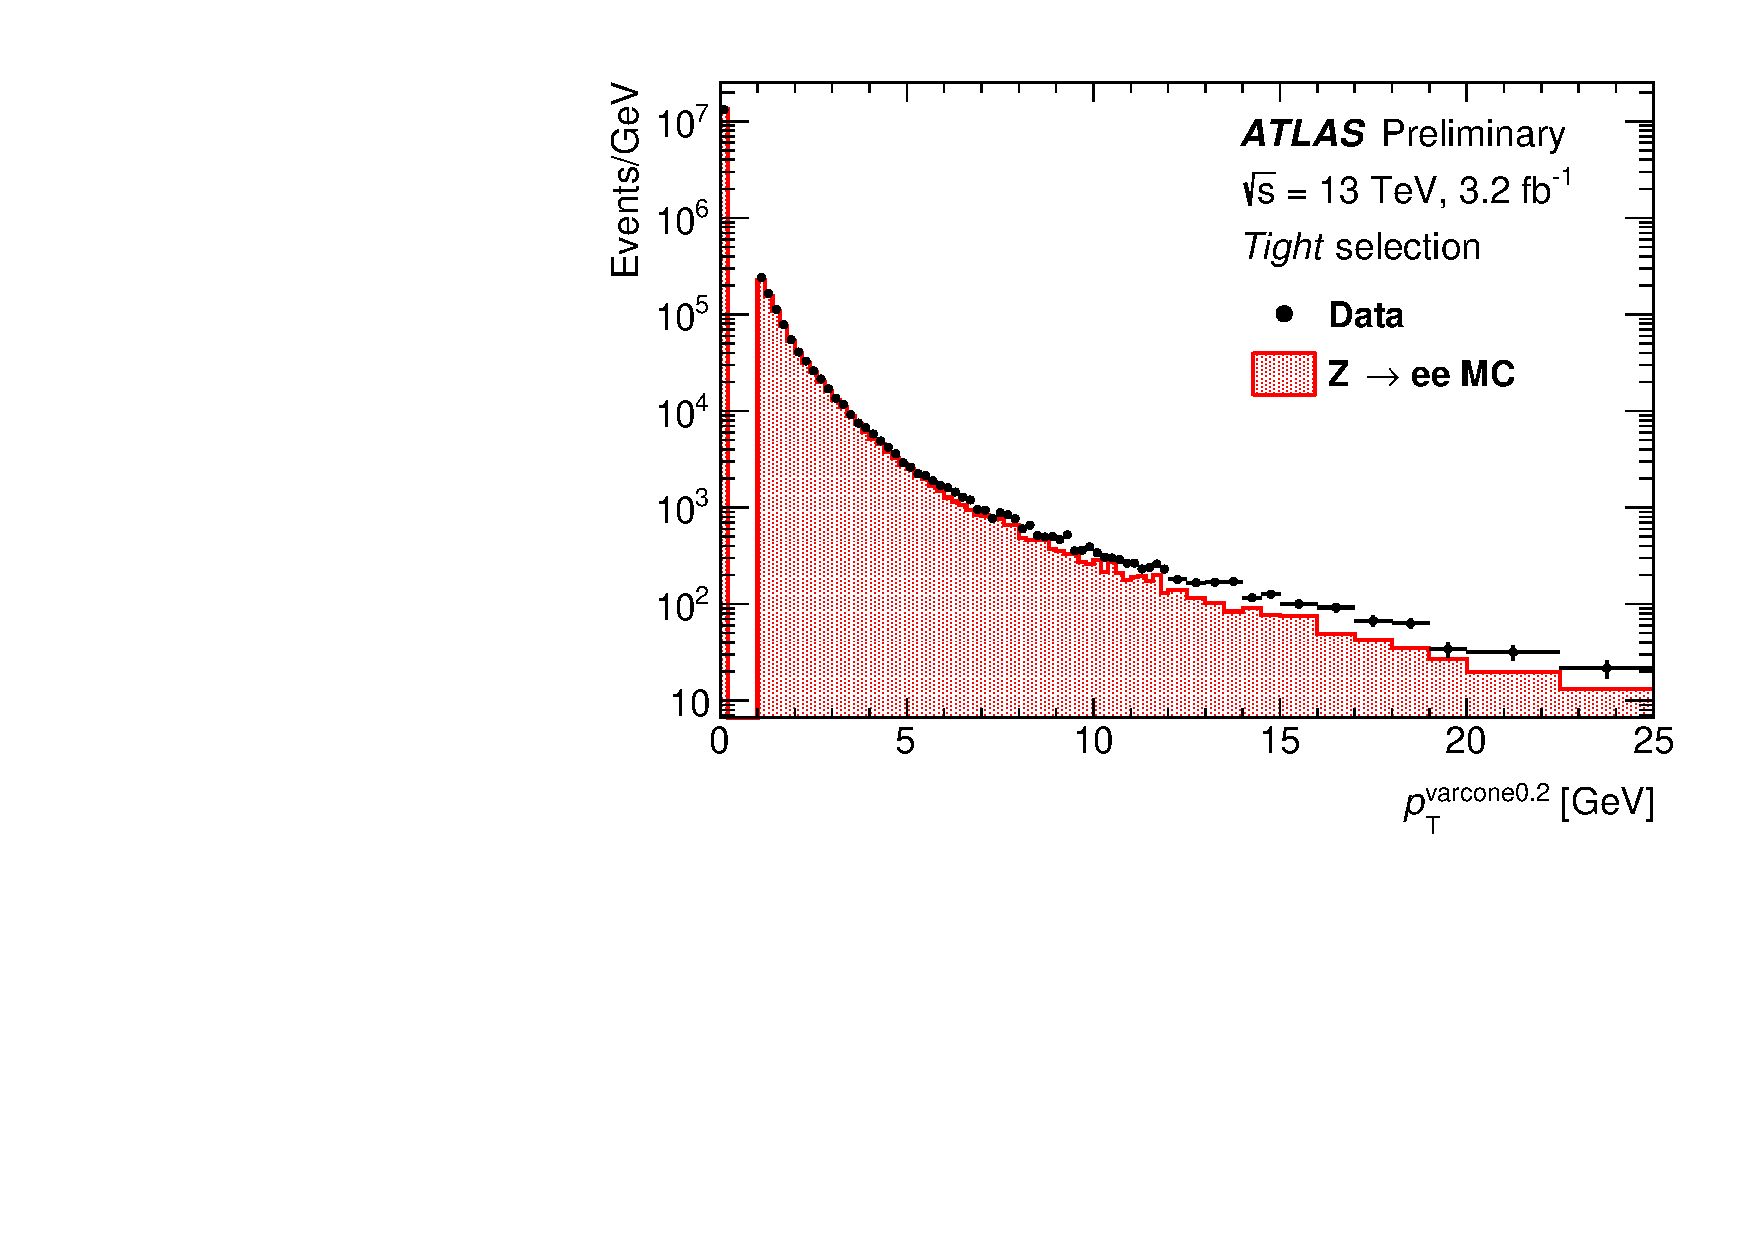
\includegraphics[scale=0.35]{fig_02b.pdf}
            \caption{$p_\mathrm{T}^\mathrm{varcone\ 0.2}$}
        \end{center}
    \end{subfigure}
    \caption{The (a) $E_\mathrm{T}^\mathrm{cone\ 0.2}$ and (b) $p_\mathrm{T}^\mathrm{varcone\ 0.2}$ distributions.
    The negative tail of $E_\mathrm{T}^\mathrm{cone\ 0.2}$ originates from the correction for pileup and the underlying event activity.
    No background subtraction is applied in the plots, so a slight discrepancy is observed in the region at large $E_\mathrm{T}^\mathrm{cone\ 0.2}$ and $p_\mathrm{T}^\mathrm{varcone\ 0.2}$ values where the background dominates.}
    \label{fig:app_electron_isolation_ETcone20_PTvarcone20}
\end{figure}

Table~\ref{tab:app_electron_isolation_working_points} lists the electron isolation working points, which are various selection requirements on the $E_\mathrm{T}^\mathrm{cone\ 0.2}$ and $p_\mathrm{T}^\mathrm{varcone\ 0.2}$, to select isolated electron candidates.
The \texttt{Tight}, \texttt{Loose}, \texttt{LooseTrackOnly}, \texttt{Gradient}, and \texttt{GradientLoose} are the efficiency targeted working points.
By applying various requirements, the isolation efficiency $\epsilon_{iso}$ can be obtained.
The \texttt{FixedCutTightTrackOnly}, \texttt{FixedCutTight}, and \texttt{FixedCutLoose} are the fixed requirement working points.
The upper thresholds on the isolation variables are constant.
The fixed requirement working points are used in analyses with low $E_\mathrm{T}$ electrons and require high background rejection.

\begin{table}[htbp]
    \begin{center}
        \resizebox{\textwidth}{!}{%
            \begin{tabular}{ccccc}
                \hline
                \hline
                Working point          & Calorimeter isolation                        & Track isolation                                 & Combined isolation\\
                \hline
                Tight                  & 96\%                                         & 99\%                                            & 95\%\\
                Loose                  & 99\%                                         & 99\%                                            & 99\%\\
                LooseTrackOnly         & -                                            & 99\%                                            & 99\%\\
                \hline
                Gradient               & $(0.1143 \times E_\mathrm{T} + 92.14)$ \%    & $(0.1143 \times E_\mathrm{T} + 92.14)$ \%       & 90\%/99\% at 25/60~{\GeV}\\
                GradientLoose          & $(0.057 \times E_\mathrm{T} + 95.57)$ \%     & $(0.057 \times E_\mathrm{T} + 95.57)$ \%        & 95\%/99\% at 25/60~{\GeV}\\
                \hline
                FixedCutTightTrackOnly & -                                            & $p_\mathrm{T}^\mathrm{varcone\ 0.2}/\pt < 0.06$ & -\\
                FixedCutTight          & $E_\mathrm{T}^\mathrm{cone\ 0.2}/\pt < 0.06$ & $p_\mathrm{T}^\mathrm{varcone\ 0.2}/\pt < 0.06$ & -\\
                FixedCutLoose          & $E_\mathrm{T}^\mathrm{cone\ 0.2}/\pt < 0.2$  & $p_\mathrm{T}^\mathrm{varcone\ 0.2}/\pt < 0.15$ & -\\
                \hline
                \hline
            \end{tabular}
        }
    \end{center}
    \caption{The definitions of the electron isolation working points.
    The numbers in the table represent the target efficiencies for the target working points.
    For Gradient, GradientLoose, and fixed requirement working points, the $E_\mathrm{T}$ and \pt are in {\GeV}.}
    \label{tab:app_electron_isolation_working_points}
\end{table}%

%%%
%%%
%%%

\section{The electron isolation efficiency}
\label{sec:app_electron_isolation_efficiency}
The probe electron candidates with $E_\mathrm{T} > 7$~{\GeV} are used in the electron isolation efficiency measurement.
The tag-and-probe method with $Z \to ee$ events are used for the efficiency measurement and the $Z_{mass}$ method is used to estimate background.
The isolation efficiency is defined as

\begin{equation}
    \epsilon_{iso} = \frac{N_{\mathrm{identification} \cap \mathrm{isolation}}}{N_\mathrm{identification}}
\end{equation}

The efficiency are measured for all isolation working points listed in Table~\ref{tab:app_electron_isolation_working_points} with respect to three likelihood identifications \texttt{TightLLH}, \texttt{MediumLLH}, and \texttt{LooseLLH}.
The electron isolation efficiencies depend on the transverse energy $E_\mathrm{T}$ and pseudorapidity $\eta$.
Fig~\ref{fig:app_electron_isolation_isolation_plots} shows the electron isolation efficiencies for the fixedCutLoose working point and data-to-MC ratios as a function of the transverse energy $E_\mathrm{T}$ and pseudorapidity $\eta$, respectively.
Larger discrepancies between data and MC are observed for $E_\mathrm{T} < 20$~{\GeV} and good agreement is found when $E_\mathrm{T} > 20$~{\GeV}.
Good agreement is also observed as a function of $\eta$ with slightly larger discrepancies at the level of 1\% in the regions $|\eta| \approx 1.5$.

\begin{figure}[htbp]
    \begin{subfigure}[b]{0.48\textwidth}
        \begin{center}
            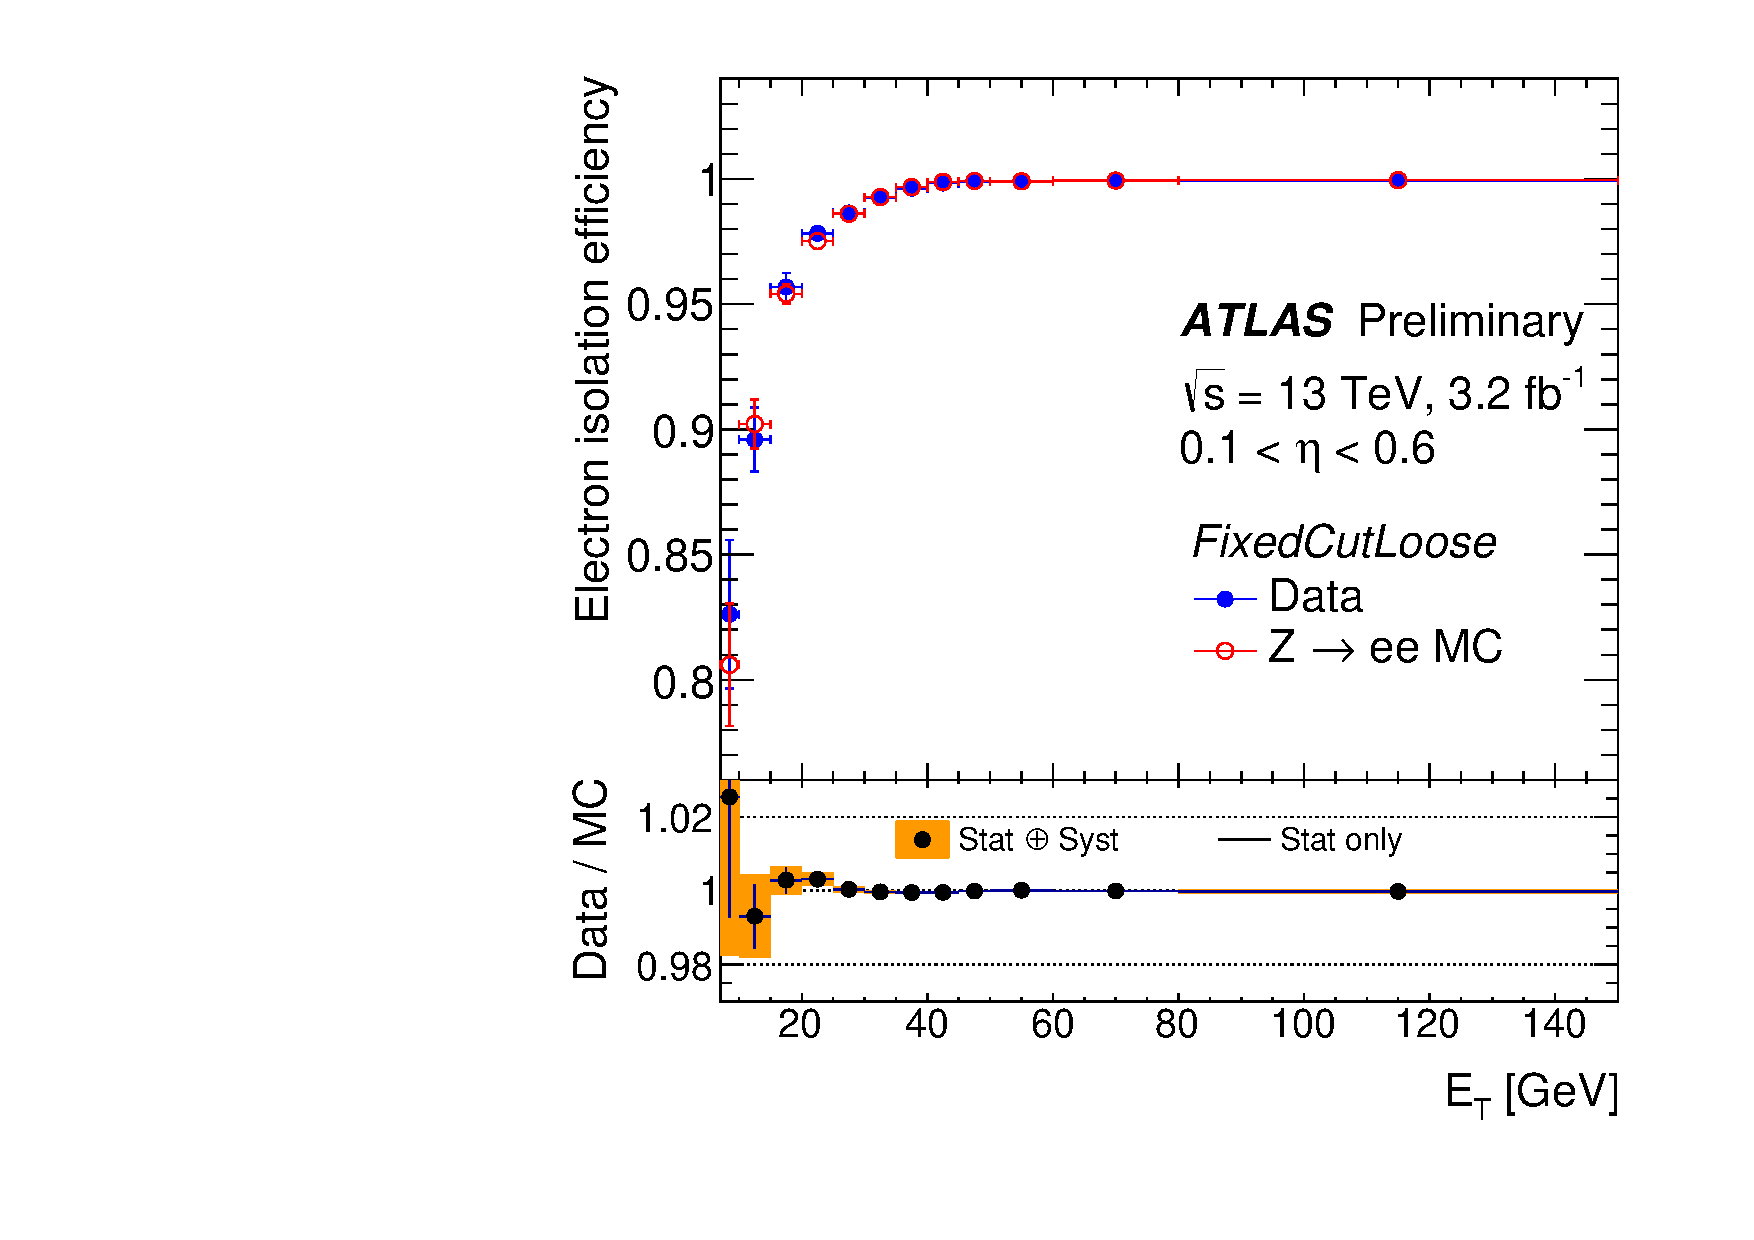
\includegraphics[scale=0.35]{fig_16a.pdf}
            \caption{The transverse energy $E_\mathrm{T}$}
        \end{center}
    \end{subfigure}
    \begin{subfigure}[b]{0.48\textwidth}
        \begin{center}
            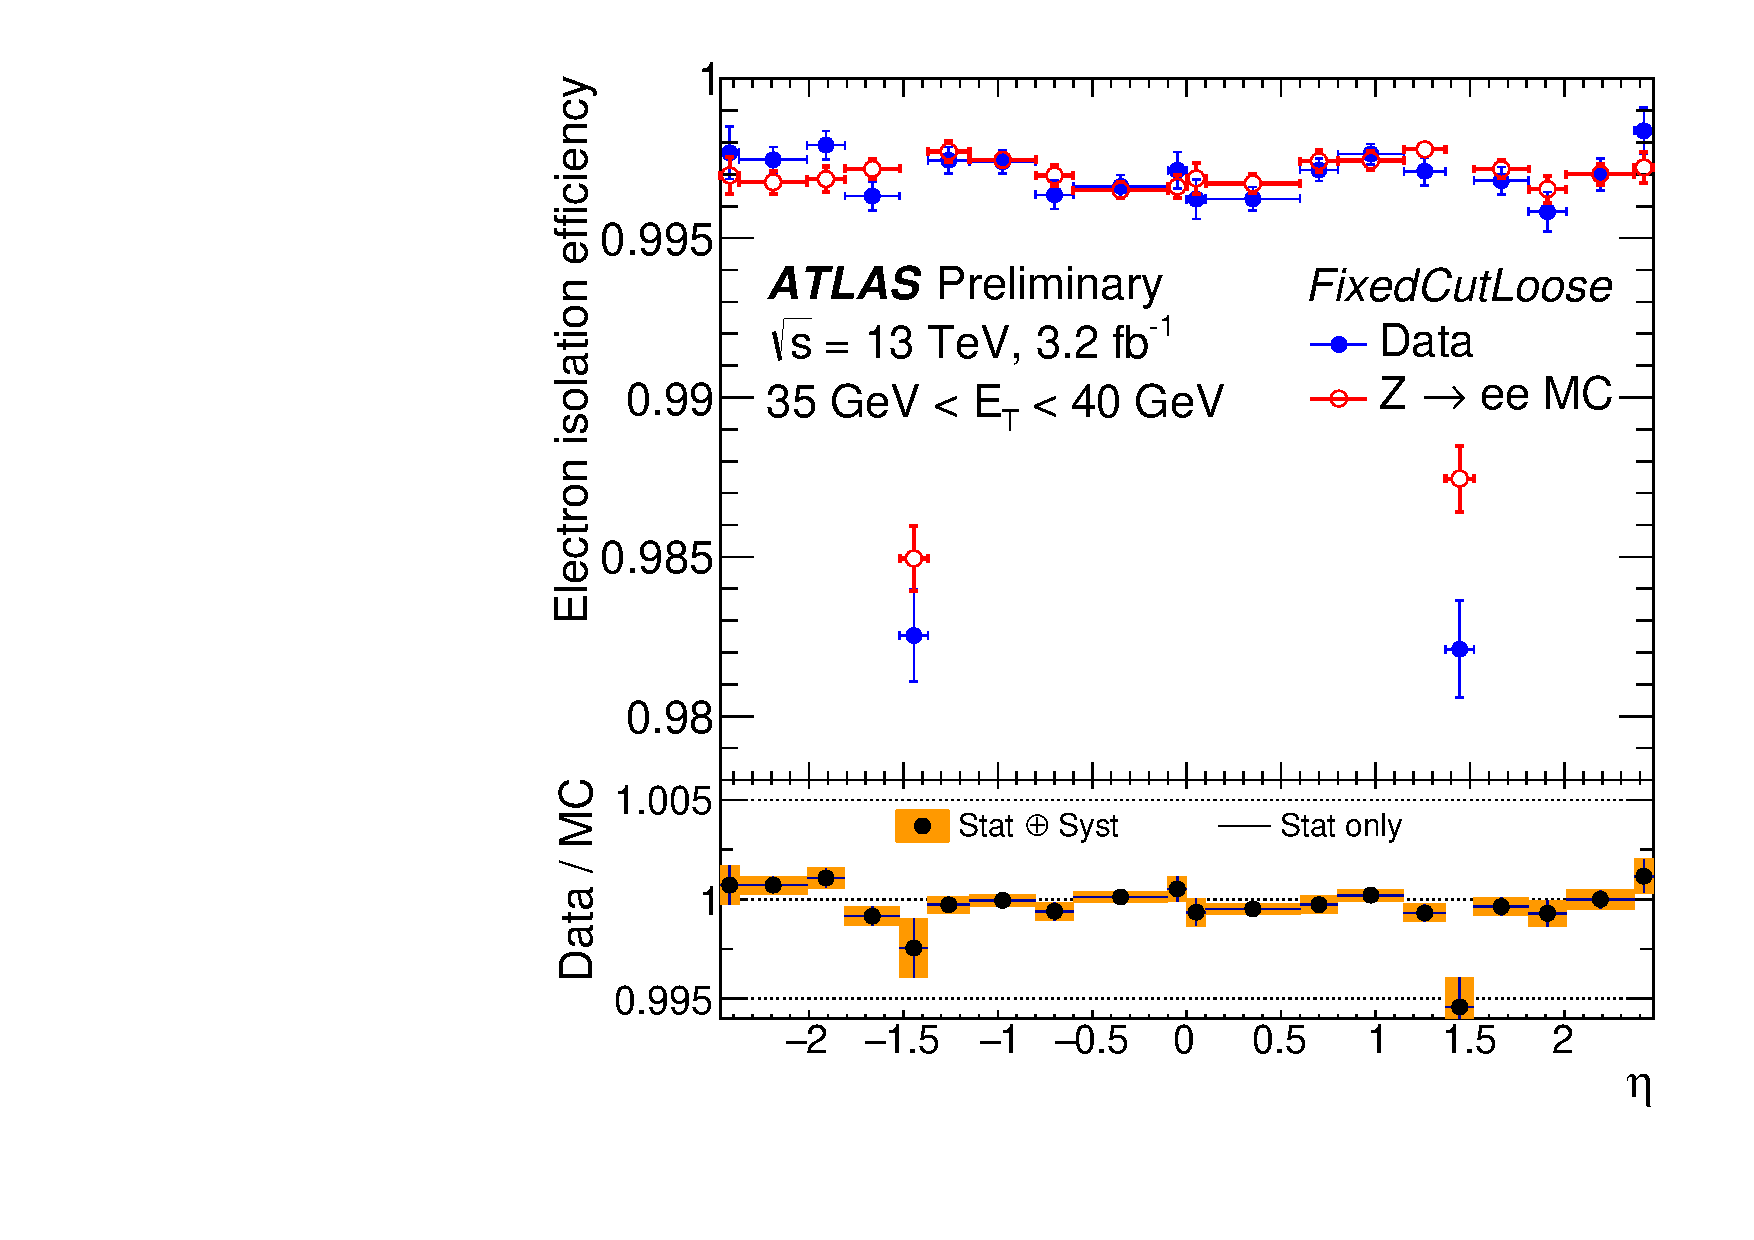
\includegraphics[scale=0.35]{fig_16b.pdf}
            \caption{$\eta$}
        \end{center}
    \end{subfigure}
    \caption{The electron isolation efficiencies for the fixedCutLoose working point for electrons from $Z \to ee$ as a function of the (a) the transverse energy $E_\mathrm{T}$ for $0.1 < \eta < 0.6$ and (b) pseudorapidity $\eta$ for $35 < E_\mathrm{T} < 40$~{\GeV}.
    The electrons are required to fulfill \texttt{TightLLH} identification.}
    \label{fig:app_electron_isolation_isolation_plots}
\end{figure}
